\subsection*{Simple function regression}

In this example we have a data set with $1$ input variable, $x$, $1$ target variable, $y$, and $101$ instances. 
The aim is to design a neural network that can predict $y$ values for given $x$ values. 
Figure \ref{SimpleFunctionRegressionDataSet} shows this data set.

\begin{figure}[!hbp]
\begin{center}
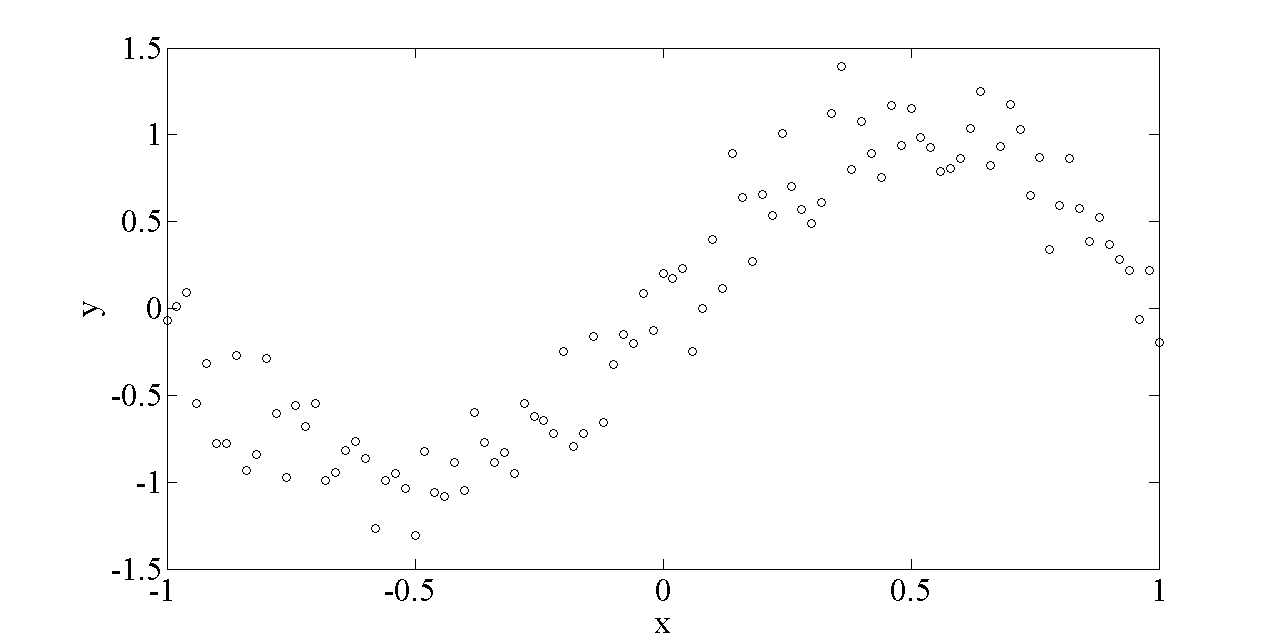
\includegraphics[width=1.0\textwidth]{function_regression/simple_function_regression_data_set.png}
\caption{Simple function regression data set.}\label{SimpleFunctionRegressionDataSet}
\end{center}
\end{figure}

Here the neural network composed of a multilayer perceptron. 
The performance functional is composed of an objective term, the normalized squared error. 
Finally, the training strategy is composed of a main training algorithm, the quasi-Newton method. 

\subsection*{Yacht resistance}

Prediction of residuary resistance of sailing yachts at the
initial design stage is of a great value for evaluating the ship's
performance and for estimating the required propulsive power.
Essential inputs include the basic hull dimensions and the boat
velocity. 
Figure \ref{SailingYatchsFigure} illustrates this example. 
That picture has been taken from Wikipedia. 

\begin{figure}[!hbp]
\begin{center}
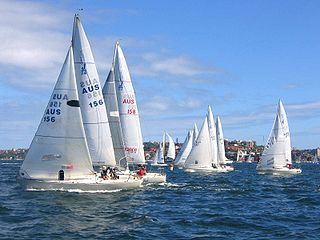
\includegraphics[width=0.7\textwidth]{function_regression/sailing_yatchs.jpg}
\caption{Sailing yatchs.}\label{SailingYatchsFigure}
\end{center}
\end{figure}

The Delft series are a semi-empirical model developed for that
purpose from an extensive collection of full-scale experiments. They
are expressed as a set of polynomials, and provide a prediction of
the residuary resistance per unit weight of displacement, with hull
geometry coefficients as variables and for discrete values of the
Froude number \cite{Gerritsma1981}. The Delft series are widely used
in the sailing yacht industry.

The Delft data set comprises 308 full-scale experiments, which were
performed at the Delft Ship Hydromechanics Laboratory
\cite{Gerritsma1981}. These experiments include 22 different hull
forms, derived from a parent form closely related to the `Standfast
43' designed by Frans Maas. 

As it has been said, variations concern hull geometry coefficients and the
Froude number:

\begin{enumerate}
\item Longitudinal position of the center of buoyancy, adimensional.
\item Prismatic coefficient, adimensional.
\item Length-displacement ratio, adimensional.
\item Beam-draught ratio, adimensional.
\item Length-beam ratio, adimensional.
\item Froude number, adimensional.
\end{enumerate}

Also, the measured variable is the residuary resistance per unit weight of
displacement:

\begin{enumerate}
\item Residuary resistance per unit weight of displacement, adimensional.
\end{enumerate}

In this example, the neural network is composed by a multilayer perceptron with scaling and unscaling layers. 
The performance functional is composed of just an objective term, the normalized squared error. 
Finally, the training strategy is only composed of a main training algorithm, the quasi-Newton method. 

\subsection*{Airfoil noise}

The noise generated by an aircraft is an efficiency and
environmental matter for the aerospace industry. An important component of the total airframe noise is the airfoil
self-noise, which is due to the interaction between an airfoil blade
and the turbulence produce in its own boundary layer and near wake.
Figure \ref{AircraftNoiseFigure} illustrates this example. 
That picture has been taken from Wikipedia. 

\begin{figure}[!hbp]
\begin{center}
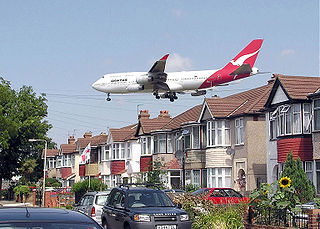
\includegraphics[width=0.7\textwidth]{function_regression/aircraft_noise.jpg}
\caption{Aircraft noise.}\label{AircraftNoiseFigure}
\end{center}
\end{figure}

The self-noise data set used in this example was processed by NASA in
1989 \cite{Brooks1989}, and so it is referred here to as the NASA
data set. It was obtained from a series of aerodynamic and acoustic
tests of two and three-dimensional airfoil blade sections conducted
in an anechoic wind tunnel. 

The NASA data set comprises different size NACA 0012 airfoils at
various wind tunnel speeds and angles of attack. The span of the
airfoil and the observer position were the same in all of the
experiments. The NASA data set contains $1503$ instances. 

In that way, this problem has the following inputs:

\begin{enumerate}
\item Frequency, in Hertzs.
\item Angle of attack, in degrees.
\item Chord length, in meters.
\item Free-stream velocity, in meters per second.
\item Suction side displacement thickness, in meters.
\item Scaled sound pressure level, in decibels.
\end{enumerate}

The only output is:

\begin{enumerate}
\item Scaled sound pressure level, in decibels.
\end{enumerate}

In this example, the neural network is composed by a multilayer perceptron with scaling and unscaling layers. 
The performance functional is composed of just an objective term, the normalized squared error. 
Finally, the training strategy is only composed of a main training algorithm, the quasi-Newton method. 

